\chapter{Introduction à la physique des réacteurs}
\section{Du processus de fission au caractéristiques d'un réacteur}
\subsection{Carburant nucléaire}
\subsubsection{Énergie produite par fission nucléaire}

	\begin{wrapfigure}[12]{l}{5cm}
	\vspace{-5mm}
	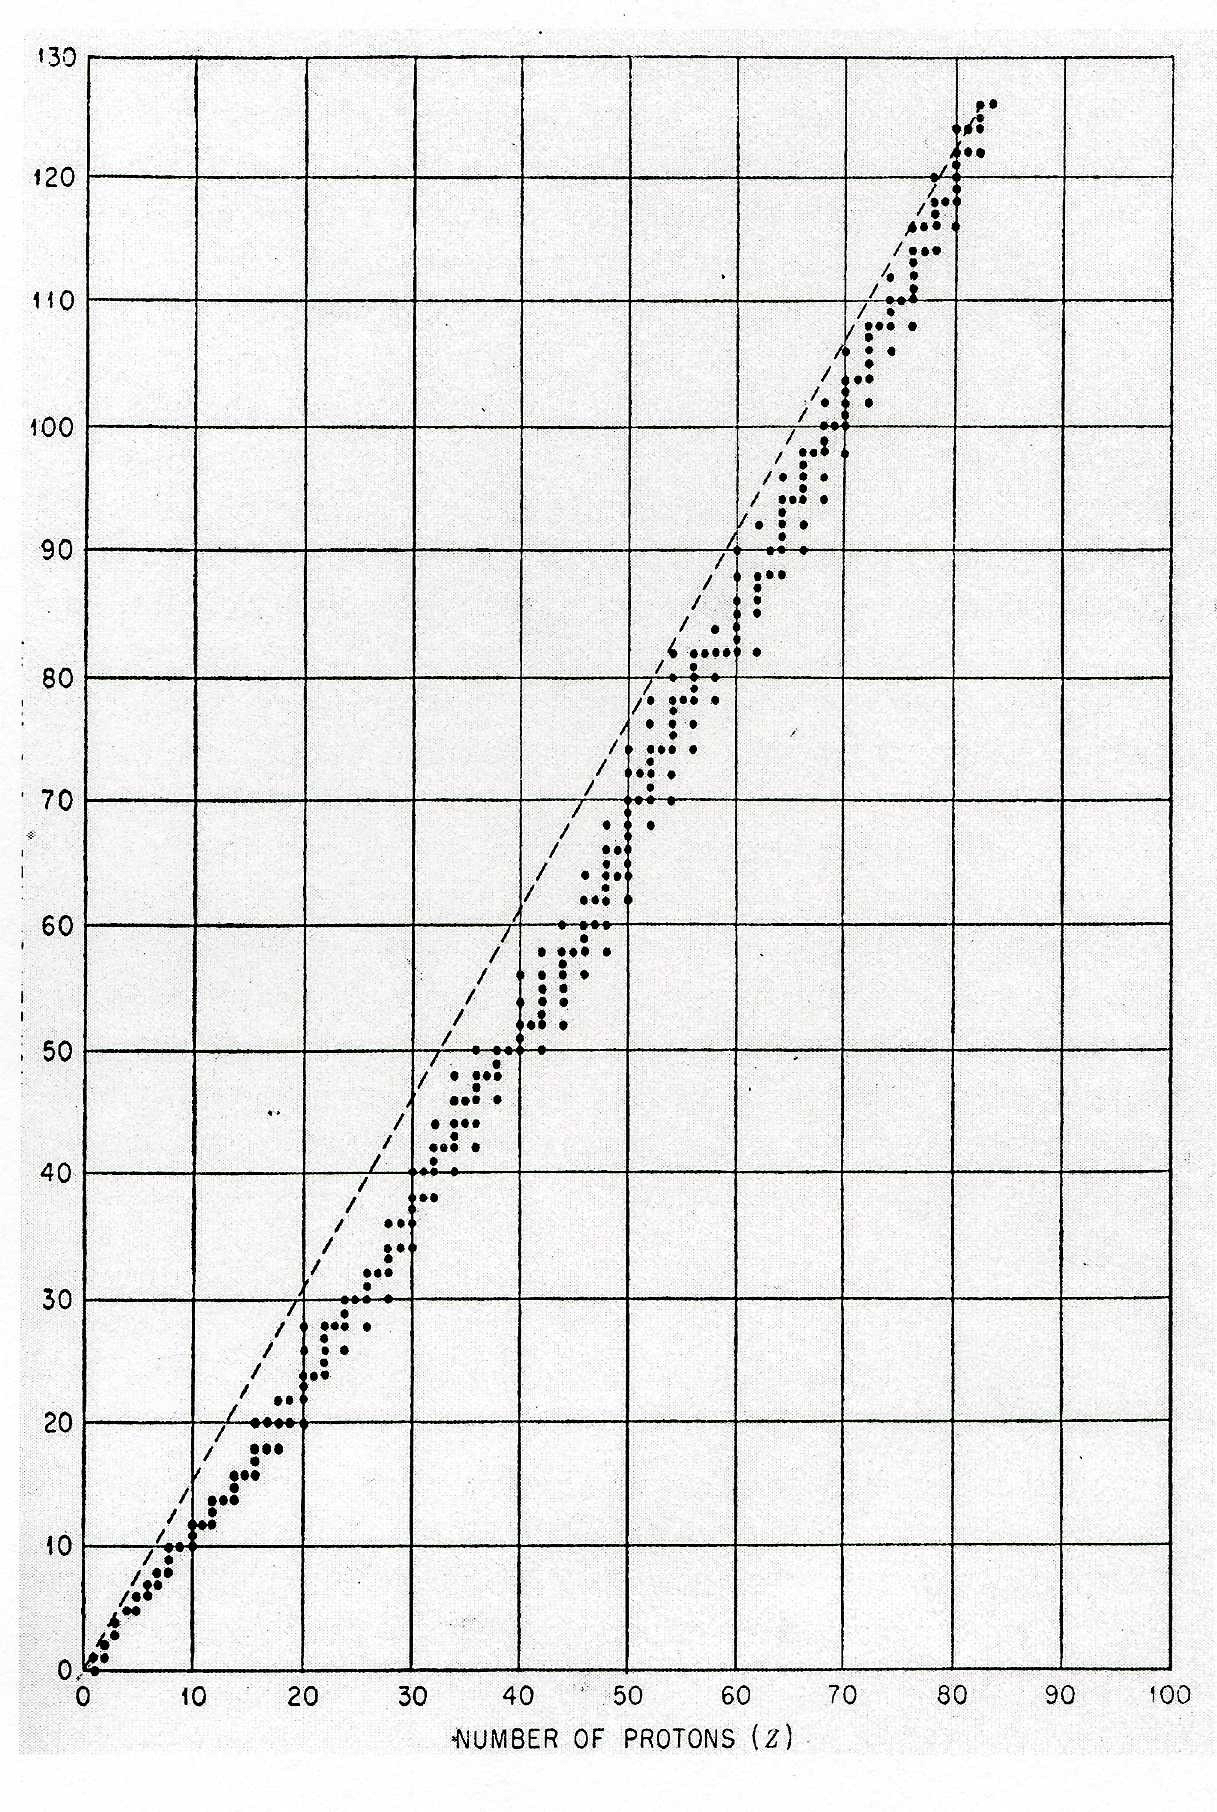
\includegraphics[scale=0.13]{ch1/image1.png}
	\captionof{figure}{ }
	\end{wrapfigure}
La stabilité des noyaux lourd est assurée par un excès du nombre de neutrons par rapport au 
nombre de protons. Le dernier élément stable est l'uranium $U$ ($Z=92$) que l'on trouve 
principalement en deux isotopes
\begin{enumerate}
\item $ ^{238}U$ $\approx$ 99.3\%
\item $ ^{235}U$ $\approx$ 0.7\%
\item $ ^{234}U$ $\approx$ traces
\end{enumerate}
Lorsque l'on observe la valée de la stabilité, on peut en effet voir que plus le nombre de 
proton augmente, plus le nombre de neutron fait de même pour stabiliser le noyau. Si un 
noyau doit se fissionner, il y aura un trop pleins de neutrons et ces derniers peuvent 
être réutiliser à certaines fins.\\ 
\\


	\begin{wrapfigure}[8]{r}{3.4cm}
	\vspace{-8mm}
	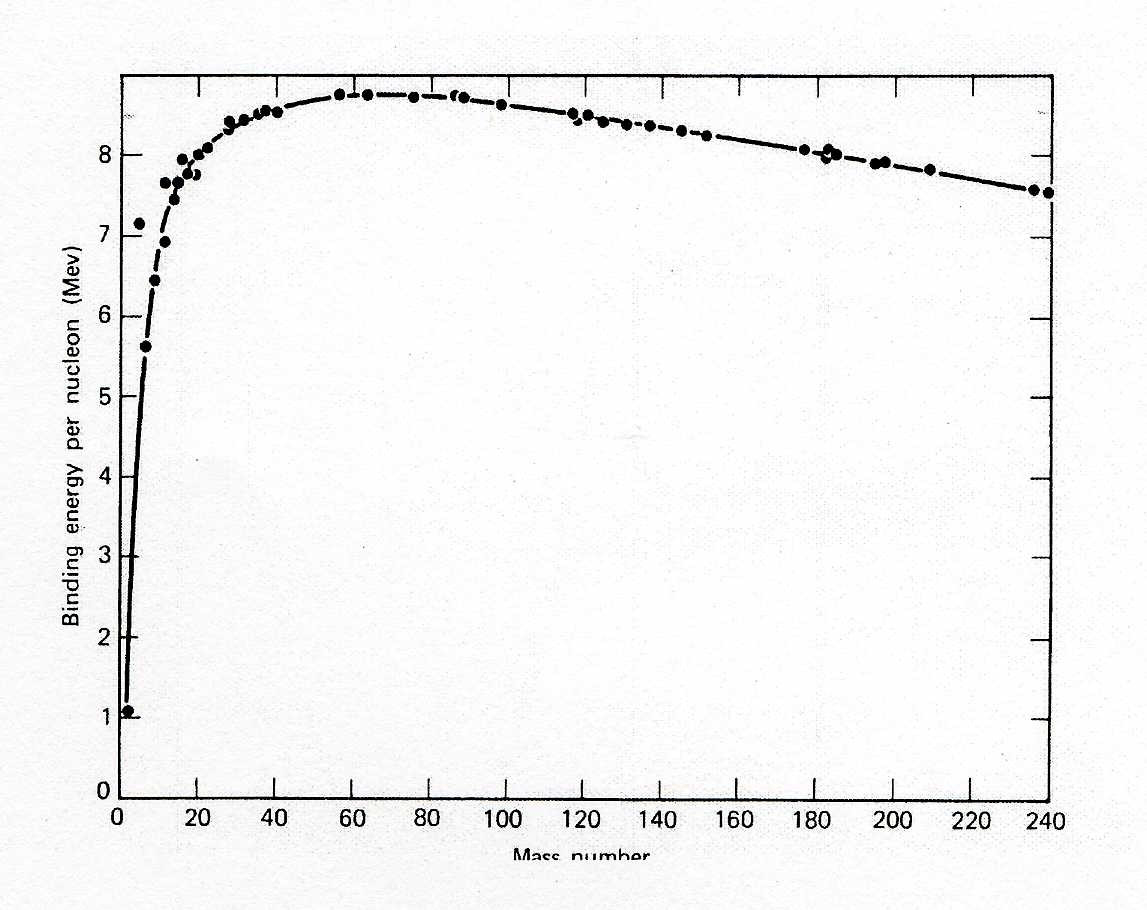
\includegraphics[scale=0.13]{ch1/image2.png}
	\captionof{figure}{ }
	\end{wrapfigure}
Une autre courbe connue est celle de l'\textit{énergie de liaison des noyaux}. Les noyaux 
possèdent un défaut de masse : la somme des masses des nucléons est plus élevée que la 
masse du noyau qu'ils constituent. Il en résulte forcéement une énergie qui a permi de 
réaliser cette liaison et c'est ce que reprend cette courbe : elle exprime cette énergie 
en fonction du nombre de masse.\\

Il existe alors deux façons de récupérer de l'énergie sur le défaut de masse. Soit en allant 
vers des noyaux qui ont un défaut de masse et récupérer cette énergie soit en fissionnant 
des noyaux lourds. 

\subsubsection{Isotopes fissiles et fertiles}
La nature n'offre pas des centaines de possibilités pour récupérer cette énergie liée au 
défaut de masse par fission : ces isotopes sont dit \textbf{fissiles} ($U_{235}$ (naturel), 
$U_{233}, Pu_{235}$. Par contre, d'autres sont dit \textbf{fertiles} : par capture neutronique, 
ils donnent lieu à un isotope fissile
\begin{equation}
\begin{array}{llll}
U_{238} + n\quad&\to\quad U_{239}+\gamma\quad&\overset{\underset{\Longrightarrow}{\text{23'}}}{\beta^-}\quad Np_{239}\quad&\overset{\underset{\Longrightarrow}{\text{2.3j}}}{\beta^-}\quad Pu_{239}
\vspace{2mm}\\
Th_{232} + n\quad&\to\quad Th_{233}+\gamma\quad&\overset{\underset{\Longrightarrow}{\text{22'}}}{\beta^-}\quad Pa_{233}\quad&\overset{\underset{\Longrightarrow}{\text{27.4j}}}{\beta^-}\quad U_{233}
\end{array}
\end{equation}
L'isotope le plus abondant de l'uranium est l'$U_{238}$ qui est forcément souvent présent dans 
les réacteurs : par ajout d'un neutron  et suite aux désintégrations $\beta$ il est possible de
créer du $Pu_{239}$ qui est fissile et s'ajoute ainsi à la matière fissile du réacteur. Hélas, 
$Pu_{239}$ est traiter comme un déchet, il n'est pas possible de l'utiliser\dots\\

De même, le thorium 232 est aussi susceptible de capturer un neutron et donner de l'uranium 233 par 
double désintégration $\beta$. On peut remarquer que les isotopes impair sont fissiles alors que les
fertiles sont pairs.\\

Le principal souci est l'abondance naturelle de $U_{235}$, seulement 0.7\%. On va alors utiliser 
de l'uranium enrichi. Pour que le réacteur fonctionne, il faudra un rapport $V/S$ choisi judicieusement afin d'éviter les fuites neutroniques et garantir une réaction en chaîne. Notons 
que l'enrichissement lié à la production d'électricité est de l'ordre que 3-4\% et de l'ordre de
plus de 90\% pour une bombe atomique.

\subsubsection{Énergie de fission}
La combustion d'un atome de carbone fourni une énergie de $3eV$ alors que la fission d'un noyau 
d'$U_{235}$ fourni 200 MeV, l'énergie susceptible d'être libérée est donc pharamineuse par rapport 
aux centrales thermiques. A partir d'un gramme d'$U_{235}$ (si fissionné entièrement) il est possible 
de fournir  1 MW durant une journée : seulement 3 kg d'$U_{235}$ sont suffisant pour faire tourner 
une centrale comme Doel 2 toute une journée.\\

Hélas, le cycle thermodynamique n'a qu'un rendement de 33\%. On distingue alors la \textit{puissance 
thermique} qui est l'énergie produite par le racteur par unité de temps (MWth) et la \textit{
puissance électrique} qui est la sortie du générateur (MWe).


\subsection{Interaction neutrons - noyaux lourds}
\subsubsection{Phénomènes possible}
Il existe plusieurs phénomènes possibles, en voici trois
\begin{enumerate}
\item \textit{Scattering}\footnote{Le scattering (diffusion) est le phénomène par lequel un rayonnement, comme la lumière, le son ou un faisceau de particules, est dévié dans diverses directions par une interaction avec d'autres objets.} du aux collisions : élastique (toute l'énergie est conservée) ou inélastique.
\item \textit{Fission}
\begin{center}
$U_{25}$ + $n$\quad$\to$\quad 2 fragments + $\gamma n + \beta + \gamma$
\end{center}
où $\nu$ est ne nombre de neutrons par fission.
\item \textit{Capture radiative}. Permet par exemple le passage de fertile à fissile
\begin{center}
$U_{25} + n\quad\to\quad U_{26}+\gamma$
\end{center}
\end{enumerate}



\subsubsection{Section efficace}
La \textbf{section efficace macroscopique} $\Sigma\ [cm^{-1}]$ est la probabilité \textbf{par unité de 
longueur\footnote{D'où le \textit{section}}} de rencontrer un type d'interaction  particulier 
dans un libre parcours dans un milieu donné. Dès lors $\Sigma$ est fonction du milieu, de 
l'énergie du neutron, de la position spatiale et, forcement, du type d'interaction.

Par exemple $\Sigma_t$ est la probabilité par unité de longueur de libre parcours 
d'avoir une interaction, quelque soit sa nature.
\begin{center}
\begin{tabular}{|c|c|}
\hline 
\multicolumn{2}{|c|}{Section efficaces en physique des réacteurs} \\ 
\hline 
\hline 
$\Sigma_{in}$ & Scattering inélastique \\ 
\hline 
$\Sigma_e$ & Scattering élastique \\ 
\hline 
$\Sigma_s = \Sigma_e+\Sigma_{in}$ & Scattering total \\ 
\hline 
$\Sigma_f$ & Fission \\ 
\hline 
$\Sigma_c$ & Capture photon $\gamma$ \\ 
\hline 
$\Sigma_a=\Sigma_c+\Sigma_f$ & Absorption (capture + fission) \\ 
\hline 
$\Sigma_t=\Sigma_a+\Sigma_s$ & Toutes les interactions \\ 
\hline 
\end{tabular} 
\end{center}


Le nombre de neutrons au bout d'un libre parcours sont ceux qui étaient déjà la moins ceux qui 
ne le sont plus
\begin{equation}
n(x+dx) = n(x)- \Sigma_t n(x) dx\quad \Leftrightarrow\quad \frac{n(x)}{n(0)} = e^{-\int_0^x \Sigma_t(x')dx'} \equiv pdf
\end{equation}
où $pdf$ signifie \textit{proba density function} (pour le libre parcours).\\

La probabilité d'une interaction dépend du nombre de noyau que l'on peut rencontrer. Il faut donc 
que la section efficace dépende de la densité atomique $[cm^{-3}]$
\begin{equation}
\Sigma = N.\sigma
\end{equation}
où $N=f(p,T)$ est la densité isotropique et $\sigma = f(noyau,\vec{v})$ la section efficace 
microscopique $[cm^2]$ qui dépend du mouvement relatif.\\


	\begin{wrapfigure}[11]{r}{4cm}
	\vspace{-8mm}
	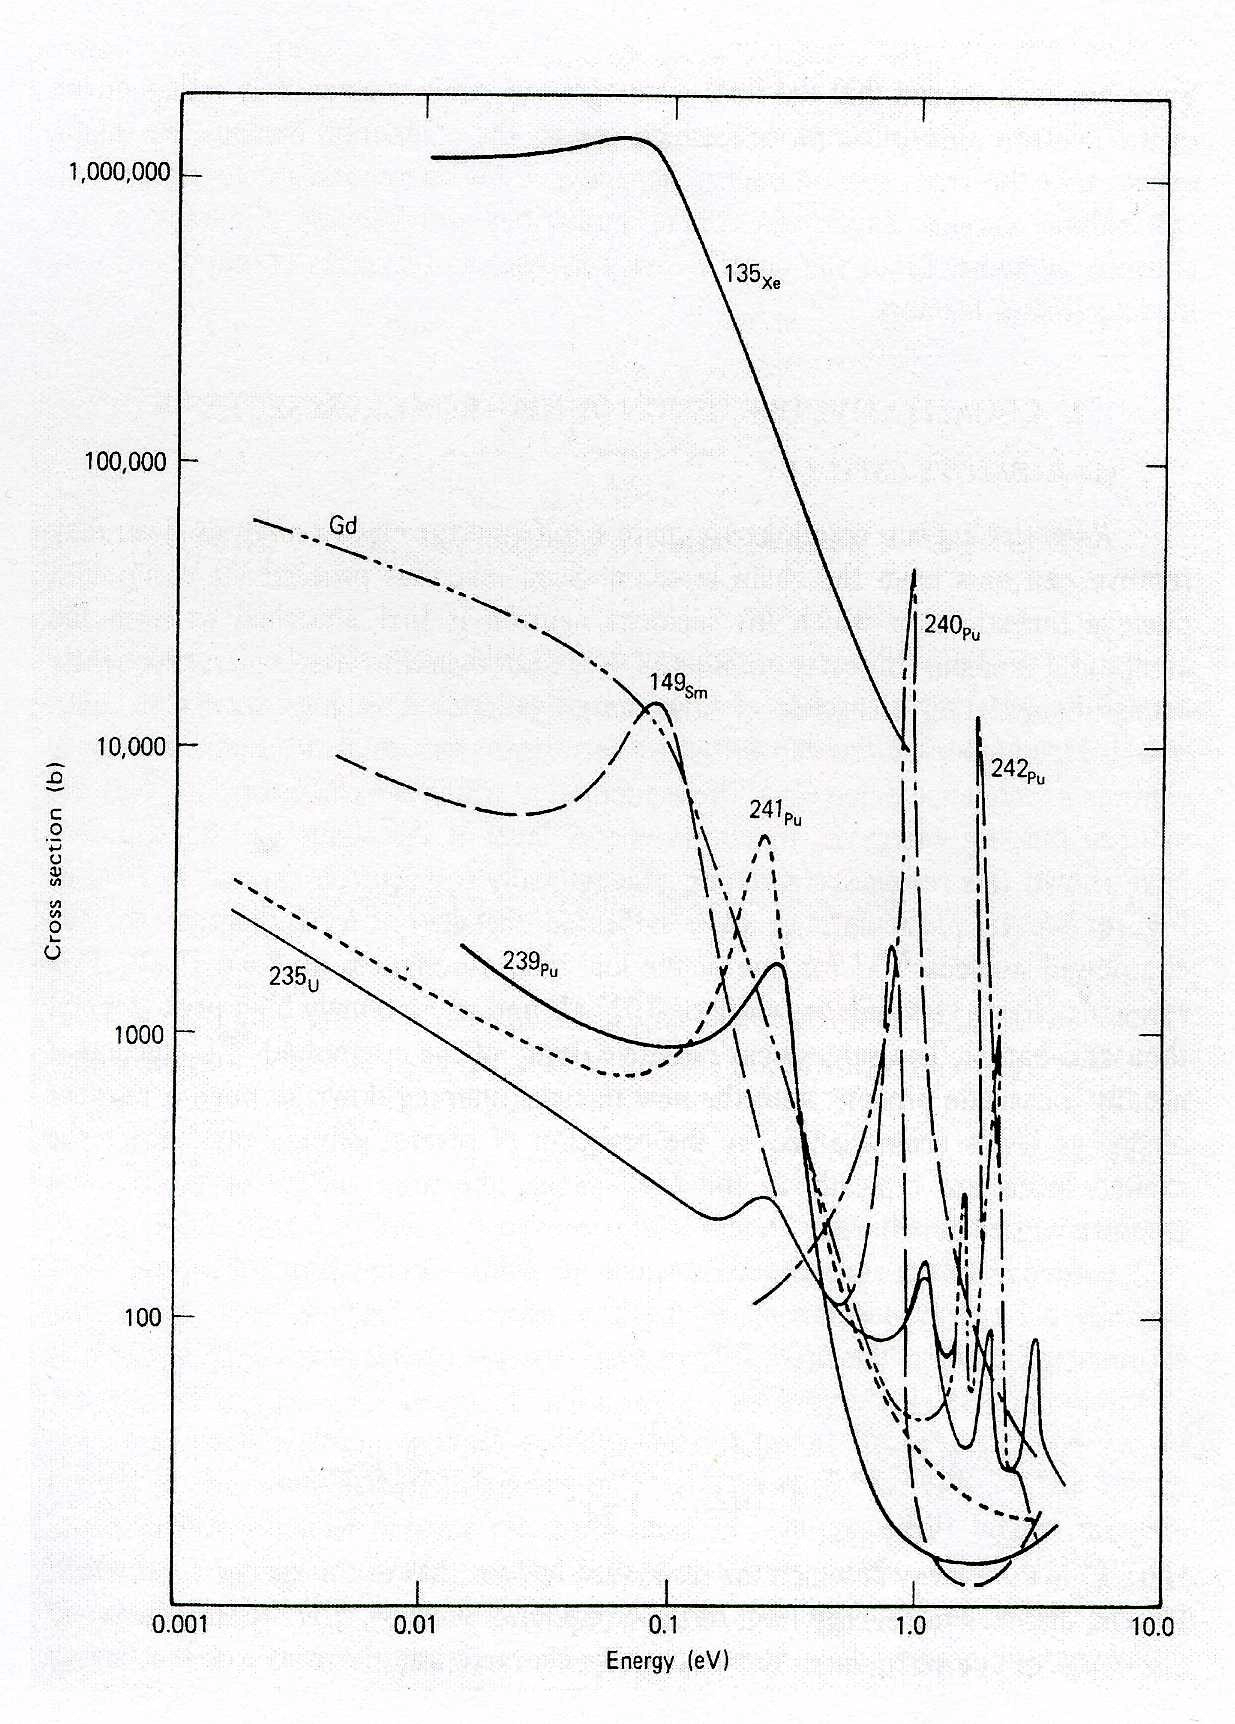
\includegraphics[scale=0.13]{ch1/image3.png}
	\captionof{figure}{ }
	\end{wrapfigure}
La section efficace est ici la section transverse (attention, même expression pour les deux en 
anglais même lorsqu'elles ne sont pas égales). On peut voir une section efficace comme un disque 
de probabilité qui peut grandir ou diminuer en fonction de la probabilité d'avoir interaction. C'est 
une notion qui remplace quelque part la section transverse géométrique.\\

Historiquement ; on imagine un neutron qui arrive face à une porte de grange (\textit{barn}) 
devant lui. On utilise alors cette unité plus adaptée : $1\ barn : 10^{-24}\ cm^2$. La section 
efficace dépend de l'énergie et l'écart entre deux phénomènes (fission et thermique) peut être 
de 8 décades.\\

Le graphique de la section efficace en fonction de l'énergie est un peu chaotique. A une température 
équivalent d'$\frac{1}{40}eV$ on retrouve des pics (résonance) : on ne parle plus de capture, 
fission, \dots \ mais de section efficace totale.\\

Regardons la gamme d'énergie que l'on peut rencontrer sur un réacteur. Un neutron émis par 
fission a une énergie d'environ 2 MeV. Or, ceci correspond à une section efficace diminuée de 
trois ordre de grandeur de ce que l'on pourrait aux énergies thermiques. Si on souhaite avoir 
de nouvelles fissions avec ces neutrons émis, il serait judicieux de les amener dans la zone 
thermique "à gauche" afin d'éviter la résonance.

\begin{center}
	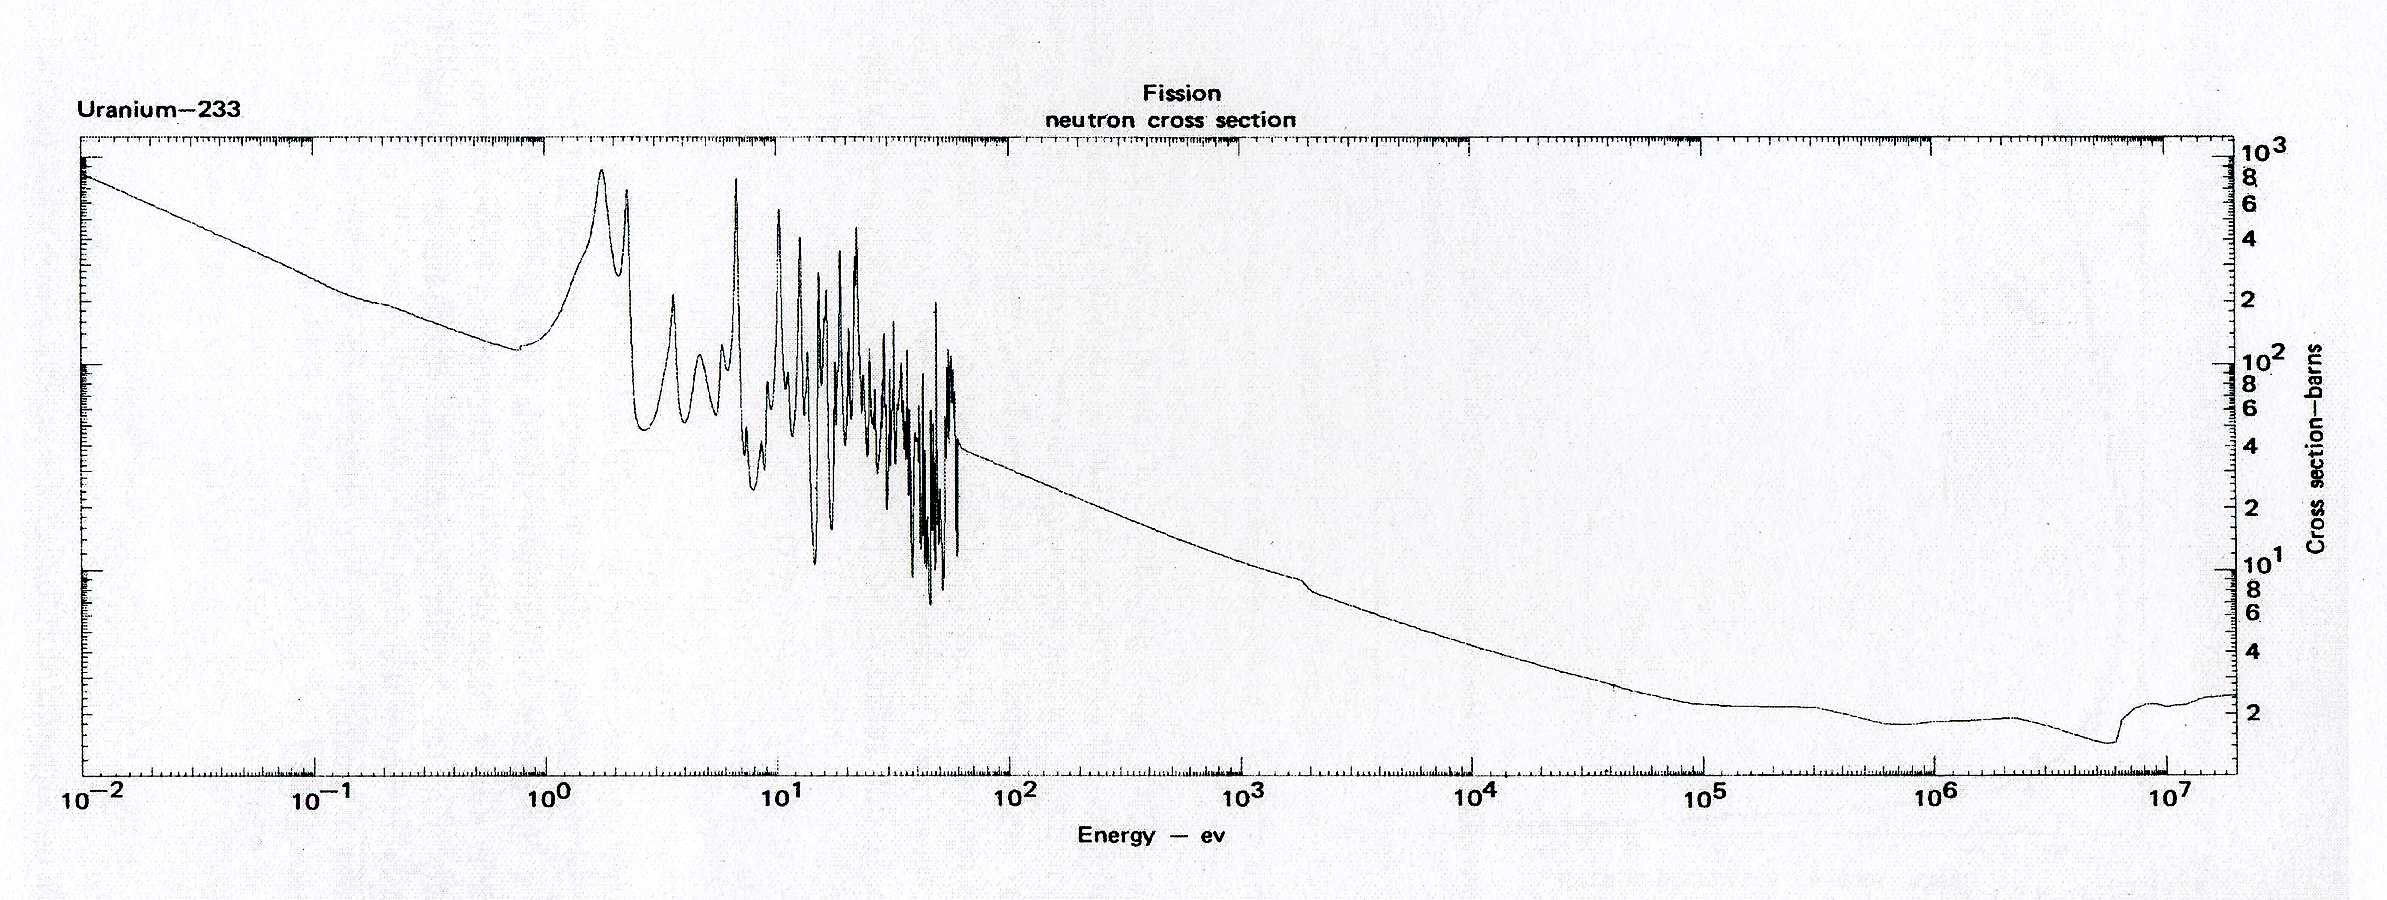
\includegraphics[scale=0.23]{ch1/image4.png}
	\captionof{figure}{ }
\end{center}

Les section efficace en terme de fission ; quand on se retrouve à l'énergie que les électrons ont après une fission, la section efficace des principaux isotopes fissibles sont 3 ordres de grandeur plus basse de ce qu'on peut avoir aux énergies thermiques. Il faut donc les refroidir suffisamment 
vite afin d'éviter qu'ils se retrouvent dans la zone dangereuse et y être mangé.\\


Pour les ralentir, il faudrait que les neutrons rentrent en collisions avec une autre "masse", de masse semblable de sorte à avoir un choc élastique. Une masse équivalent au neutron est le proton, 
on va alors utiliser l'eau (fluide caloporteur) qui va également jouer le rôle de ralentisseur de 
neutron pour un réacteur thermique afin qu'il soit suffisamment ralenti (et donc avec moins 
d'énergie) pour se trouver "a gauche" des résonance lors de sa collision avec un noyau lourd. On 
parle de \textit{neutrons thermiques}



\begin{center}
	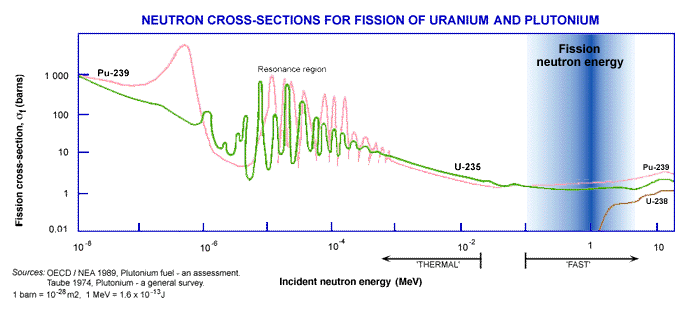
\includegraphics[scale=0.7]{ch1/image5.png}
	\captionof{figure}{ }
\end{center}

Il existe tout de même une petite marge pour tout de même faire autre chose : maintenir les énergies 
assez élevée afin de produire plus de matière fissile que ce qui a été consommé. En effet, si on 
parvient à légèrement monter les énergies il sera possible de fissionner l'$U_{238}$ qui produira 
de la nouvelle matière fissile, le $Pu_{239}$. On parle de \textit{neutrons rapides}. Pour les 
accélérer il ne faut pas utiliser de l'eau mais des éléments lourds.























\iffalse
\subsection{Cycle neutronique et criticité}
\subsection{Éléments constitutif d'un réacteur}
\fi